%!TEX root = main.tex
\subsection{A3C}
The algorithm we used to beat the baseline is the asynchronous advantage actor-critic (A3C) algorithm proposed by Volodymyr et al.~\cite{mnih2016asynchronous}. It is a policy-based model-free reinforcement learning method. This algorithm maintains a policy $\pi (a_{t}|s_{t};\theta)$ and the estimate of the value function $V(s_{t};\theta_{v})$, where $\theta$ and $\theta_{v}$ are the parameters. These two parameters are learned by taking the gradient of $\log \pi (a_{t}|s_{t};\theta) A(s_{t},a_{t};\theta,\theta_{v})$ with respect to $\theta^{\prime}$. The update of $\pi (a_{t}|s_{t};\theta)$ and $V(s_{t};\theta_{v})$ happens either after every $t_{max}$ actions or when a terminal state is reached. Combining with the idea in deep learning, we use a convolutional neural network that has one softmax output for the policy $\pi (a_{t}|s_{t};\theta)$ and one linear output for the value function $V(s_{t};\theta_{v})$.


\subsection{Policy Gradient}
The objective function:
\begin{equation*}
\begin{split}
\min_{\theta}\sum_{t=1}^N R_t (-\sum_{i=1}^{n}\textbf{I}(a_i, a_t)\log(\pi(a_i|s_t; \theta))
\end{split}
\end{equation*}
where $N$ is the number of time step in one episode, $n$ is the number of actions
in action space, $\textbf{I}(x, y)$ is an indicator function defined as $\textbf{I}(x, y) = 1 \text{ if } x==y \text{ else } 0$.

The architecture of policy gradient. 

\begin{figure}[h!]
\label{fig:pg_picture}
\centering
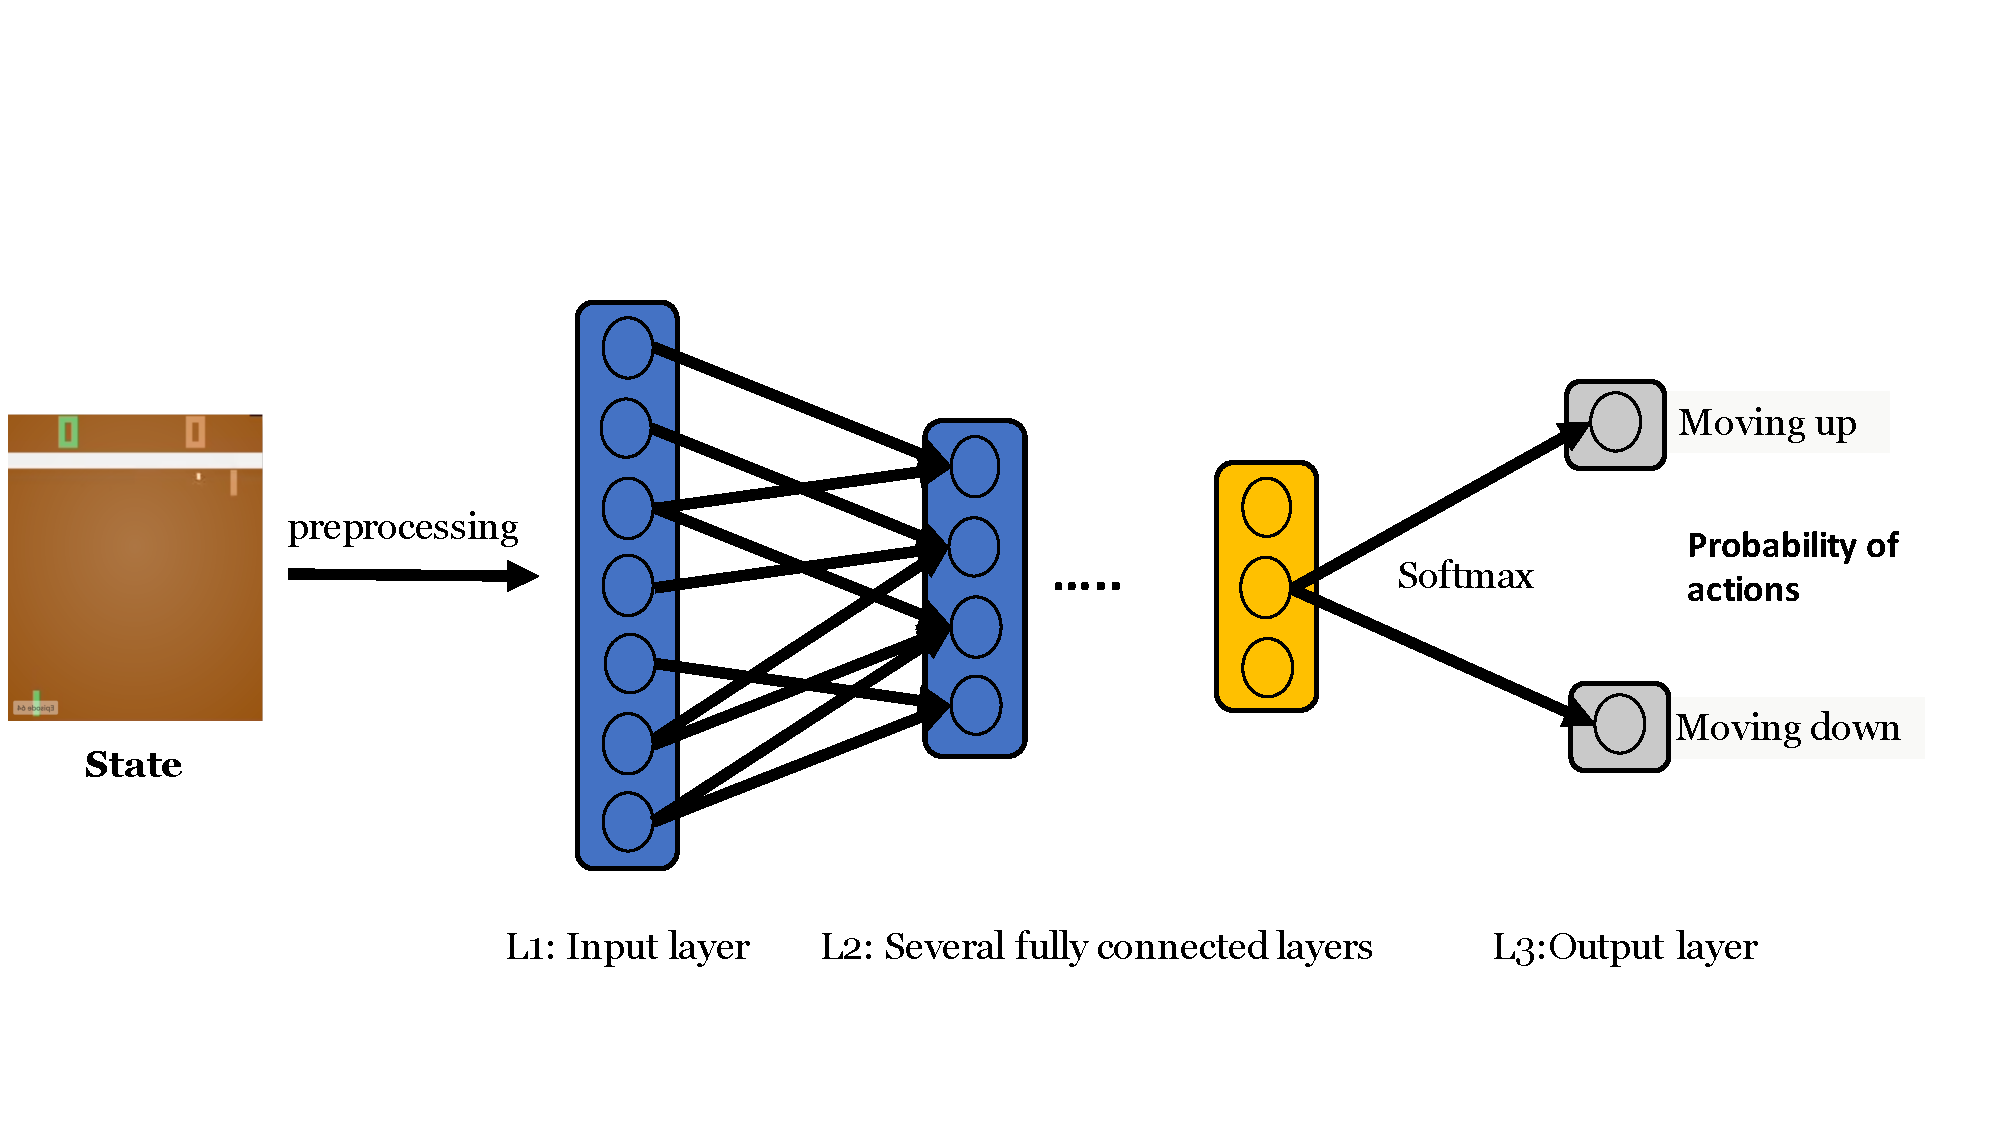
\includegraphics[width=0.49\textwidth]{./fig/policygradient.pdf} \\
\caption{The architecture of policy gradient, using Pong game as an example.}
\end{figure}


The algorithm of policy gradient:

\begin{algorithm}[H]
\begin{algorithmic}[1]
\STATE Xavier initialization: Initialize the weight parameters
\WHILE{$i=1$ to $N$}
\STATE Preprocessing 
\STATE Policy forward
\STATE Sample action, receive reward
\STATE Policy gradient
\IF{Finish one batch:} 
\STATE Rmsprop/Adam optimizer update
\ENDIF
\ENDWHILE
\end{algorithmic}
\caption{pseudocode for Policy Gradient }
\label{alg:pseudocode Pong}
\end{algorithm}

% The derive of objective function:

% \begin{equation}
% \begin{split}
% & \max_{\theta} \textbf{E}_a(R(a))  \\
% & \max_{\theta} \sum_a p(a|s; \theta)R(a)
% \end{split}
% \end{equation}
% maximize the expectation of rewards over actions